\documentclass[a4paper,12pt]{article}
\usepackage{geometry}
 \geometry{
 a4paper,
 total={170mm,257mm},
 left=20mm,
 top=20mm,
 }
\usepackage[export]{adjustbox} %% for picture frame
\usepackage[english]{babel}
\usepackage[utf8]{inputenc}
\usepackage{fancyhdr}

%%%question enviroment 

%%% Question Environment%%%  use 
%%% Question Environment%%%  use 
%%% Question Environment%%%  use \input{./QueENV.tex}   to include
%% Use \begin{Q}....\end{Q}

\newcounter{QC}
\setcounter{QC}{1}
\newenvironment{Q}[1]{
    \section{Question -\arabic{QC}} \stepcounter{QC}{\large\textbf{#1}}
}

%%% Question Environment%%%

   to include
%% Use \begin{Q}....\end{Q}

\newcounter{QC}
\setcounter{QC}{1}
\newenvironment{Q}[1]{
    \section{Question -\arabic{QC}} \stepcounter{QC}{\large\textbf{#1}}
}

%%% Question Environment%%%

   to include
%% Use \begin{Q}....\end{Q}

\newcounter{QC}
\setcounter{QC}{1}
\newenvironment{Q}[1]{
    \section{Question -\arabic{QC}} \stepcounter{QC}{\large\textbf{#1}}
}

%%% Question Environment%%%



\pagestyle{fancy}
\fancyhf{}
\rhead{\textit{LAB-1}}
\lhead{\textit{Pul074BEX004}}
\rfoot{\thepage}

%%% format and command for lab ans c and assembly

%%% Formating And Command for Embedded Lab   Assambly & C%%%


%%% Formatting And Command for Embedded Lab   Assembly & C%%%
%% 
%%% Formating And Command for Embedded Lab   Assambly & C%%%


%%% Formatting And Command for Embedded Lab   Assembly & C%%%
%% 
%%% Formating And Command for Embedded Lab   Assambly & C%%%


%%% Formatting And Command for Embedded Lab   Assembly & C%%%
%% \input{./asm c.tex}

%% \anscode{problem no. like 1,2,3...}{assembly code file }{ code file}


\usepackage{listings}
\usepackage{multicol}
\usepackage{mdframed}

\renewcommand{\lstlistlistingname}{List of Codes}
\renewcommand{\lstlistingname}{Code}


\setlength{\columnsep}{0.5cm}

\usepackage{xcolor}
\definecolor{codegreen}{rgb}{0,0.6,0}
\definecolor{codegray}{rgb}{0.4,0.4,0.4}
\definecolor{codepurple}{rgb}{0.58,0,0.82}
%\definecolor{backcolour}{rgb}{0.95,0.99,0.92}
\definecolor{backcolour}{rgb}{0,0,0}


\lstdefinestyle{customa}{
  backgroundcolor=\color{backcolour},   commentstyle=\color{codegreen},
  keywordstyle=\color{magenta},
  numberstyle=\tiny\color{codegray},
  stringstyle=\color{codepurple},
  basicstyle=\ttfamily\small\color{white},
  breakatwhitespace=false,
  breaklines=true,
  captionpos=b,
  morekeywords={MOV,ADD,ADDC,ACALL,INC,DJNZ,AJMP,RET,END,ORG,RR,JNC,SUBB,JC,DEC,ANL,SWAP,MUL,DIV,CLR,SETB},
  keepspaces=true,
  numbers=left,
  numbersep=5pt,
  showspaces=false,
  showstringspaces=false,
  showtabs=false,
  tabsize=4
}

\lstdefinestyle{customc}{
  backgroundcolor=\color{backcolour},   commentstyle=\color{codegreen},
  keywordstyle=\color{cyan},
  numberstyle=\tiny\color{codegray},
  stringstyle=\color{codepurple},
  basicstyle=\ttfamily\footnotesize\color{white},
  breakatwhitespace=false,
  breaklines=true,
  captionpos=b,
  keepspaces=true,
  language=C,
  numbers=left,
  numbersep=5pt,
  showspaces=false,
  showstringspaces=false,
  showtabs=false,
  tabsize=3
}




\newcommand {\anscode}[3]{

  \begin{center}
    \textbf{Assembly}
  \end{center}

  \begin{multicols}{2}
    \lstinputlisting[style=customa,nolol]{#2}
  \end{multicols}

  \begingroup
  \captionof{lstlisting}{Problem no. #1 Assembly}
  \endgroup


  \vspace{2 em}


  \begin{center}
    \textbf{C language }
  \end{center}
  \begin{multicols}{2}
    \lstinputlisting[style=customc,nolol]{#3}
  \end{multicols}

  \begingroup
  \captionof{lstlisting}{Problem no. #1 C language}
  \endgroup
}

%%% Formating And Command for Embedded Lab  Assambly & C%%%

%% \anscode{problem no. like 1,2,3...}{assembly code file }{ code file}


\usepackage{listings}
\usepackage{multicol}
\usepackage{mdframed}

\renewcommand{\lstlistlistingname}{List of Codes}
\renewcommand{\lstlistingname}{Code}


\setlength{\columnsep}{0.5cm}

\usepackage{xcolor}
\definecolor{codegreen}{rgb}{0,0.6,0}
\definecolor{codegray}{rgb}{0.4,0.4,0.4}
\definecolor{codepurple}{rgb}{0.58,0,0.82}
%\definecolor{backcolour}{rgb}{0.95,0.99,0.92}
\definecolor{backcolour}{rgb}{0,0,0}


\lstdefinestyle{customa}{
  backgroundcolor=\color{backcolour},   commentstyle=\color{codegreen},
  keywordstyle=\color{magenta},
  numberstyle=\tiny\color{codegray},
  stringstyle=\color{codepurple},
  basicstyle=\ttfamily\small\color{white},
  breakatwhitespace=false,
  breaklines=true,
  captionpos=b,
  morekeywords={MOV,ADD,ADDC,ACALL,INC,DJNZ,AJMP,RET,END,ORG,RR,JNC,SUBB,JC,DEC,ANL,SWAP,MUL,DIV,CLR,SETB},
  keepspaces=true,
  numbers=left,
  numbersep=5pt,
  showspaces=false,
  showstringspaces=false,
  showtabs=false,
  tabsize=4
}

\lstdefinestyle{customc}{
  backgroundcolor=\color{backcolour},   commentstyle=\color{codegreen},
  keywordstyle=\color{cyan},
  numberstyle=\tiny\color{codegray},
  stringstyle=\color{codepurple},
  basicstyle=\ttfamily\footnotesize\color{white},
  breakatwhitespace=false,
  breaklines=true,
  captionpos=b,
  keepspaces=true,
  language=C,
  numbers=left,
  numbersep=5pt,
  showspaces=false,
  showstringspaces=false,
  showtabs=false,
  tabsize=3
}




\newcommand {\anscode}[3]{

  \begin{center}
    \textbf{Assembly}
  \end{center}

  \begin{multicols}{2}
    \lstinputlisting[style=customa,nolol]{#2}
  \end{multicols}

  \begingroup
  \captionof{lstlisting}{Problem no. #1 Assembly}
  \endgroup


  \vspace{2 em}


  \begin{center}
    \textbf{C language }
  \end{center}
  \begin{multicols}{2}
    \lstinputlisting[style=customc,nolol]{#3}
  \end{multicols}

  \begingroup
  \captionof{lstlisting}{Problem no. #1 C language}
  \endgroup
}

%%% Formating And Command for Embedded Lab  Assambly & C%%%

%% \anscode{problem no. like 1,2,3...}{assembly code file }{ code file}


\usepackage{listings}
\usepackage{multicol}
\usepackage{mdframed}

\renewcommand{\lstlistlistingname}{List of Codes}
\renewcommand{\lstlistingname}{Code}


\setlength{\columnsep}{0.5cm}

\usepackage{xcolor}
\definecolor{codegreen}{rgb}{0,0.6,0}
\definecolor{codegray}{rgb}{0.4,0.4,0.4}
\definecolor{codepurple}{rgb}{0.58,0,0.82}
%\definecolor{backcolour}{rgb}{0.95,0.99,0.92}
\definecolor{backcolour}{rgb}{0,0,0}


\lstdefinestyle{customa}{
  backgroundcolor=\color{backcolour},   commentstyle=\color{codegreen},
  keywordstyle=\color{magenta},
  numberstyle=\tiny\color{codegray},
  stringstyle=\color{codepurple},
  basicstyle=\ttfamily\small\color{white},
  breakatwhitespace=false,
  breaklines=true,
  captionpos=b,
  morekeywords={MOV,ADD,ADDC,ACALL,INC,DJNZ,AJMP,RET,END,ORG,RR,JNC,SUBB,JC,DEC,ANL,SWAP,MUL,DIV,CLR,SETB},
  keepspaces=true,
  numbers=left,
  numbersep=5pt,
  showspaces=false,
  showstringspaces=false,
  showtabs=false,
  tabsize=4
}

\lstdefinestyle{customc}{
  backgroundcolor=\color{backcolour},   commentstyle=\color{codegreen},
  keywordstyle=\color{cyan},
  numberstyle=\tiny\color{codegray},
  stringstyle=\color{codepurple},
  basicstyle=\ttfamily\footnotesize\color{white},
  breakatwhitespace=false,
  breaklines=true,
  captionpos=b,
  keepspaces=true,
  language=C,
  numbers=left,
  numbersep=5pt,
  showspaces=false,
  showstringspaces=false,
  showtabs=false,
  tabsize=3
}




\newcommand {\anscode}[3]{

  \begin{center}
    \textbf{Assembly}
  \end{center}

  \begin{multicols}{2}
    \lstinputlisting[style=customa,nolol]{#2}
  \end{multicols}

  \begingroup
  \captionof{lstlisting}{Problem no. #1 Assembly}
  \endgroup


  \vspace{2 em}


  \begin{center}
    \textbf{C language }
  \end{center}
  \begin{multicols}{2}
    \lstinputlisting[style=customc,nolol]{#3}
  \end{multicols}

  \begingroup
  \captionof{lstlisting}{Problem no. #1 C language}
  \endgroup
}

%%% Formating And Command for Embedded Lab  Assambly & C%%%
%%%%>>>>>>>........
%%%%%% include  Titles.%%%% use \input{./CP}%%%
%%%use """"""""    \CP{}{}{}{}   """" %%%% and 4 argument to craete Title page 
%%%%%%%%%%%%%%%%%%%%%%%%%%%%%%%%%%%%%%%%%%%%%%%%%%%%%%%%%%%%%%%%%
%%%argument number
%% 1=major header ## Course name 
%% 2=minor4 heading ## lab/assignmet no
%% 3=Title  ## Assignment or Lab title
%% 4=submitted to::## input receiver Name"
%%%%%%%%%%%%%%%%%%%%%%%%%%%%%%%%%%%%%%%%%%%%%%%%%%%%%%%%%%%%%%%%%


\usepackage{mathpazo} % Palatino font
\usepackage{graphicx}
\usepackage{float}

%%% format and command for lab ans c and assembly

\newcommand{\HRule}{\rule{\linewidth}{0.4mm}} % Defines a new command for horizontal lines, change thickness here



%----------------------------------------------------------------------------------------
%	TITLE PAGE
%----------------------------------------------------------------------------------------


\newcommand{\CP}[4]{ \begin{titlepage} % Suppresses displaying the page number on the title page and the subsequent page counts as page 1
		%%%%  univerdity logo%%
		\begin{figure}[H]
			\centering
			
\includegraphics[scale=0.13]{tulogo.jpg}
		\end{figure}
		%%% end university logo

		\center % Centre everything on the page

		%------------------------------------------------
		%	Headings
		%------------------------------------------------

		\textsc{\huge Institute of Engineering \\ Central Campus,Pulchowk}\\[1.5cm] % Main heading such as the name of your university/college

		\textsc{\Large #1}\\[0.5cm] % Major heading such as course name

		\textsc{\large #2}\\[0.5cm] % Minor heading such as assignment no./ lab no.

		%------------------------------------------------
		%	Title
		%------------------------------------------------

		\HRule\\[0.4cm]

		{\Huge\bfseries #3}\\[0.4cm] % Title of your document

		\HRule\\[1.5cm]

		%------------------------------------------------
		%	Author(s)
		%------------------------------------------------
		\vfill\vfill
		\begin{minipage}{0.4\textwidth}
			\begin{flushleft}
				\large{
				\textbf{Submitted BY:}\\
				{\normalsize AMRIT PRASAD PHUYAL}\\ % NAME
				{\normalsize Roll: PULL074BEX004}} % Roll
			\end{flushleft}
		\end{minipage}
		~
		\begin{minipage}{0.4\textwidth}
			\begin{flushright}
				\large
				\textbf{Submitted To:}\\
				{ \normalsize{#4}\\ }% recepent's  Name 
				{\normalsize Department of Electronics and Computer Engineering}
			\end{flushright}
		\end{minipage}

		%------------------------------------------------
		%	Date
		%------------------------------------------------

		\vfill\vfill\vfill % Position the date 3/4 down the remaining page

		{\large\today} % Date, change the \today to a set date if you want to be precise

		\vfill % Push the date up 1/4 of the remaining page

	\end{titlepage}
}

\begin{document}

%----------------------------------------------------------------------------------------
%	TITLE PAGE
%----------------------------------------------------------------------------------------
\CP{Embedded system}{LAB \#1}
{ Familiarization with 8051/8052 Microcontroller}
{Department of Electronics and Computer Engineering}




%----------------------------------------------------------------------------------------
\pagenumbering{gobble}
\tableofcontents
\pagebreak
\listoffigures
\pagebreak
\pagenumbering{arabic}
\section{Introduction} 
\subsection{Microcontroller}
A microcontroller is an integrated circuit ( IC), usually via an MPU, memory and certain peripherals, to control other parts of an electronic system . 
These devices are optimized for embed-in applications that require agile and agile processing, digital, analog or electromechanical interactions.
\subsection{8051 Microcontroller}
In 1981, Intel introduced an 8-bit microcontroller called the 8051. It was referred as system on a chip because it had 128 bytes of RAM, 4K byte of on-chip ROM,
 two timers, one serial port, and 4 ports (8-bit wide), all on a single chip.\\\\
The different features of the 8051 microcontroller include:
\begin{itemize}
\item 4KB bytes on-chip program memory (ROM)
\item 128 bytes on-chip data memory (RAM)
\item Four register banks
\item 128 user defined software flags
\item 8-bit bidirectional data bus
\item 16-bit unidirectional address bus
\item 32 general purpose registers each of 8-bit
\item 16 bit Timers (usually 2, but may have more or less)
\item Three internal and two external Interrupts
\item Four 8-bit ports,(short model have two 8-bit ports)
\item 16-bit program counter and data pointer
\item 8051 may also have a number of special features such as UARTs, ADC, Op-amp, etc.
\end{itemize}
\begin{figure}
	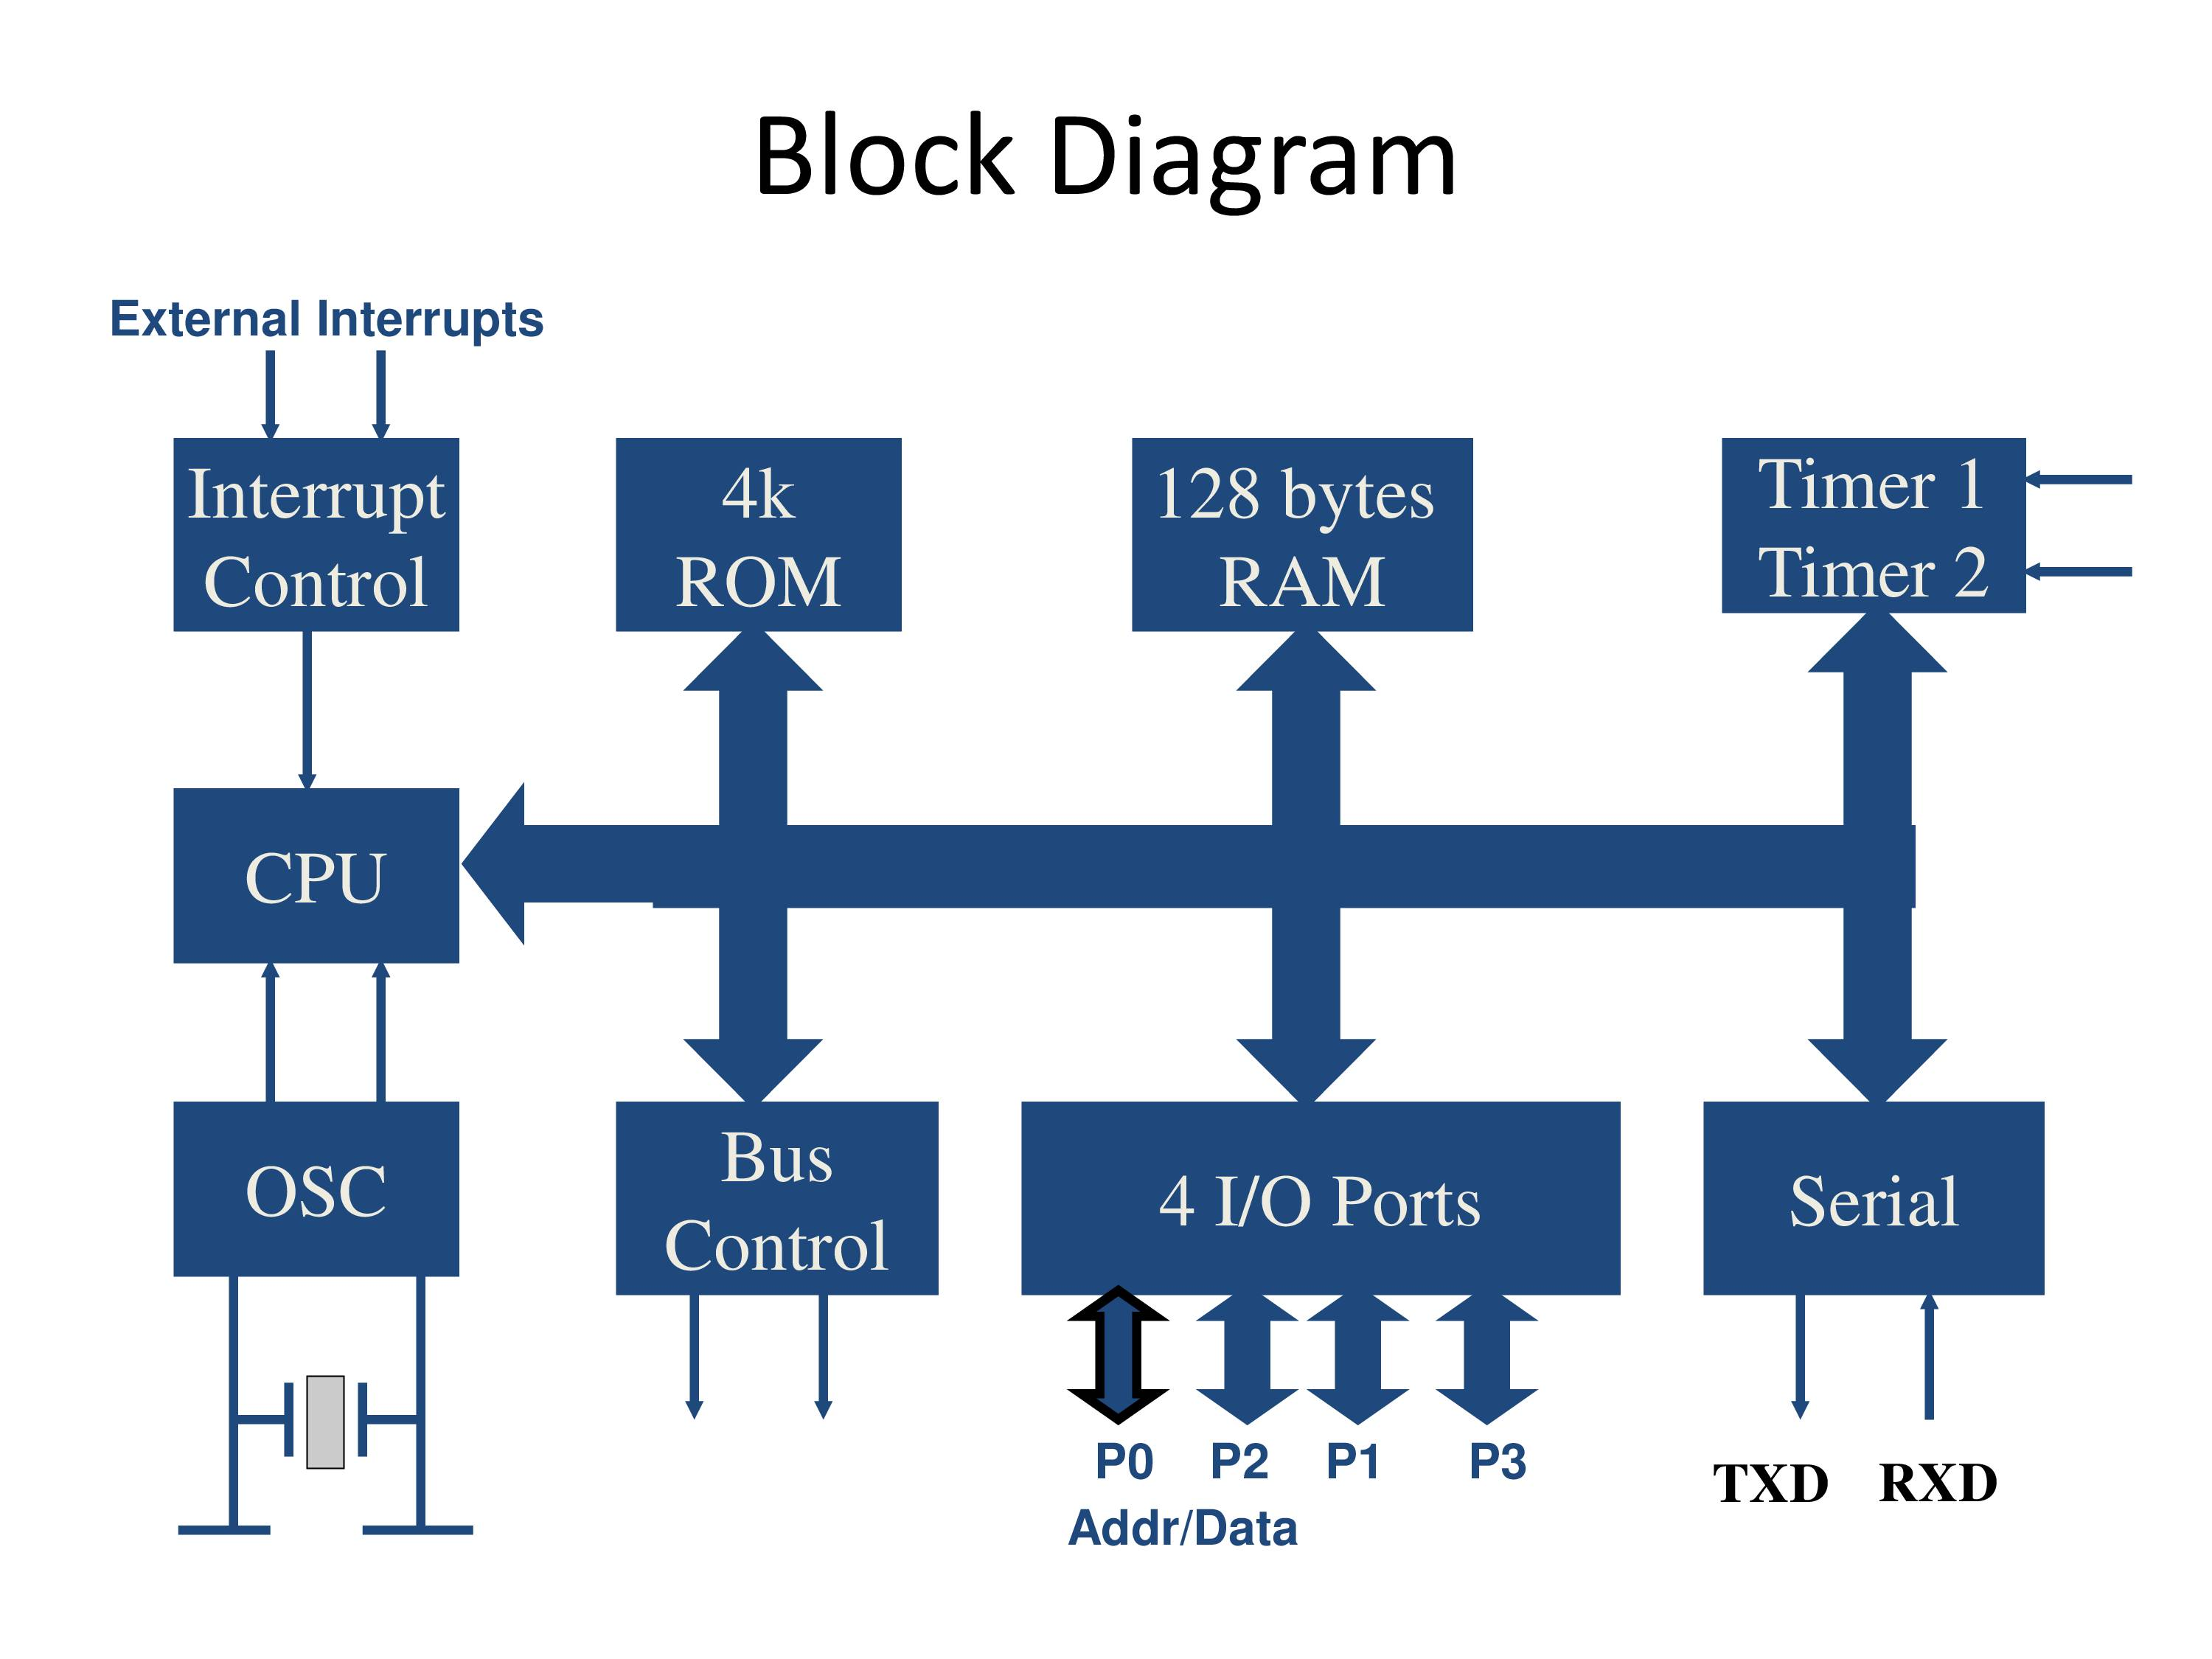
\includegraphics[scale=0.615,cframe=blue 0.5pt 3pt]{./block_diagram.jpg} 
	\textit{\caption{Block diagram of 8051 microcontroller}}

\end{figure}


\subsubsection{Memory Architecture}
 Internal RAM, Program Memory, External Data Memory, and Special Function Registers are Four different typre of memeory  available in 8051 microcontroller.The Internal RAM, 
 or generally referred to as the IRAM has an 8-bit address space taking up the addressess from 0x00 to 0xFF.Program memory, referred as PMEM is up to 64 KB of read-only memory, 
 starting at address 0 in a separate address space.XRAM is a third address space memory space starting at address 0 with 16-bit address space.
 SFR are located at the same address as IRAM i.e. at 0x80 to 0xFF and accessed just as lower half of IRAM. 

\subsubsection{Programming}
8051 can be programmed using both assembly language or embedded C language . In assembly language  mnemonics  along with hex codes is used ,
 has faster execution and has more control over the  memory than in high level language like C, which is more like human readable English language.
\subsubsection{Applications of 8051 Microcontroller}
Even with the development of many advanced and superior Microcontrollers, 8051 Microcontroller is still being used in many embedded system and applications.\\\\

Some of the applications of 8051 Microcontroller are mentioned below: 
\begin{itemize}
\item Consumer Appliances (TV Tuners, Remote controls, Computers, Sewing Machines, etc.)
\item Home Applications (TVs, VCR, Video Games, Camcorder, Music Instruments, Home Security Systems, Garage Door Openers, etc.)
\item Communication Systems (Mobile Phones, Intercoms, Answering Machines, Paging Devices, etc.)
\item Office (Fax Machines, Printers, Copiers, Laser Printers, etc.)
\item Automobiles (Air Bags, ABS, Engine Control, Transmission Control, Temperature Control, Keyless Entry, etc)
\item Aeronautical and Space
\item Medical Equipment
\item Defense Systems
\item Robotics
\item Industrial Process and Flow Control
\item Radio and Networking Equipment
\item Remote Sensing
\end{itemize}

\section{Objectives of Lab- 1}
 Familiarization with the 8051/8052 microcontroller will enable us to write assembly language code for the 8051/8052 microcontroller capble of:
\begin{itemize}
\item Data manipulation
\item Looping and branching techniques
\item Arthimetic and logical operations
\item Subroutine calls
\end{itemize}
\section{Lab Experiment Environment}
The lab experiments will be performed virtually via various simulation software. 
The fundamental use of these tools allows the different functional units of the 8051 micro controller to be visualized and defined to do simple logical and arthemetic work.
 For this lab Proteus design suite for simlulation  and KEIl IDE are used .

\begin{figure}[H]
	\centering
	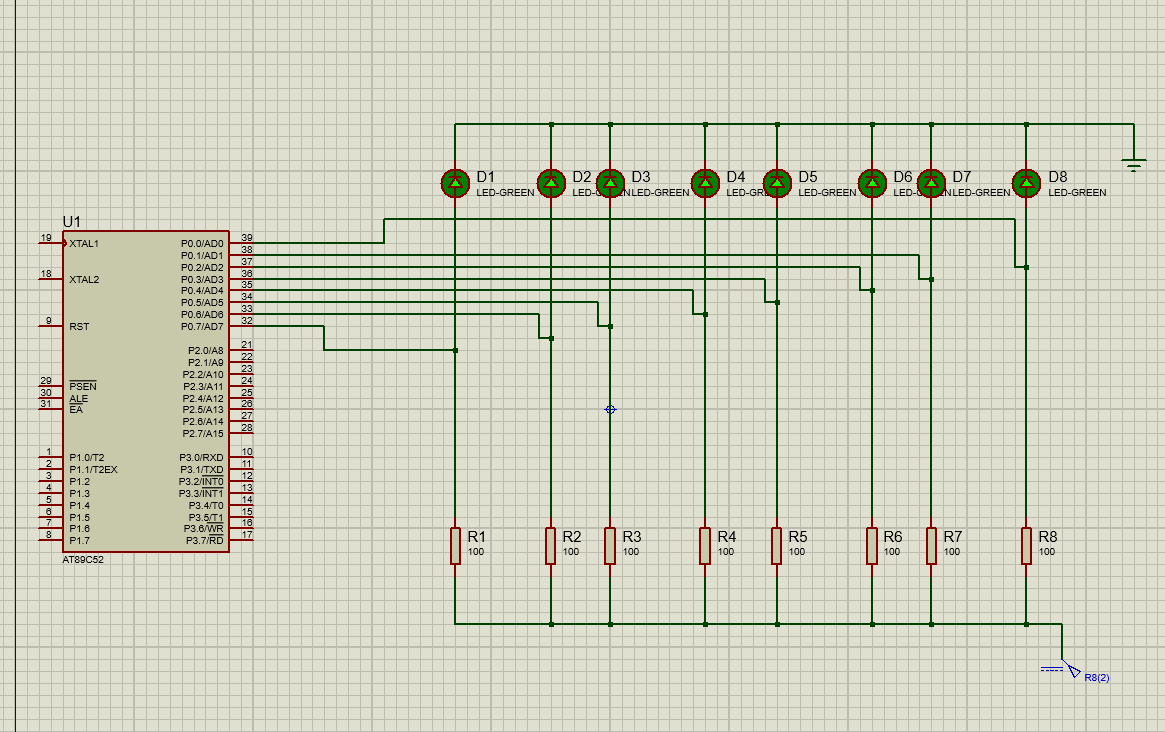
\includegraphics[scale=0.40,cframe=blue 0.5pt 3pt]{./proteus.png} 
	\textit{\caption{Proteus simulation}}

\end{figure}

\newpage 
\large\textbf{Lab Problems}
%%%%%%%%111111%%%%%
\begin{Q}
	{Write code to add the numbers 897F9AH and 34BC48H and save the result in internal RAM starting
	at 40H. The result should be displayed continuously on the LEDs of the development board starting
	from least significant byte with an appropriate timing interval between each byte. Use port zero (P0)
	of the micro-controller to interface with LEDs.}
\end{Q}

\anscode{1a.asm}{1b.c}
\pagebreak

\textbf{OUTPUT :\\}

For all output  port 0 values are snapshot from keil ide using breakpoint feature.
For this particular problem, additional IRAM and snapshot of proteus are included.
The addition of 897F9AH and 34BC48H gives 00BE3BE2H which is continuously displayed on Port 0 
and stored at 40H starting from LSB, which can be viewed in IRAM table.


\begin{figure}[H]
	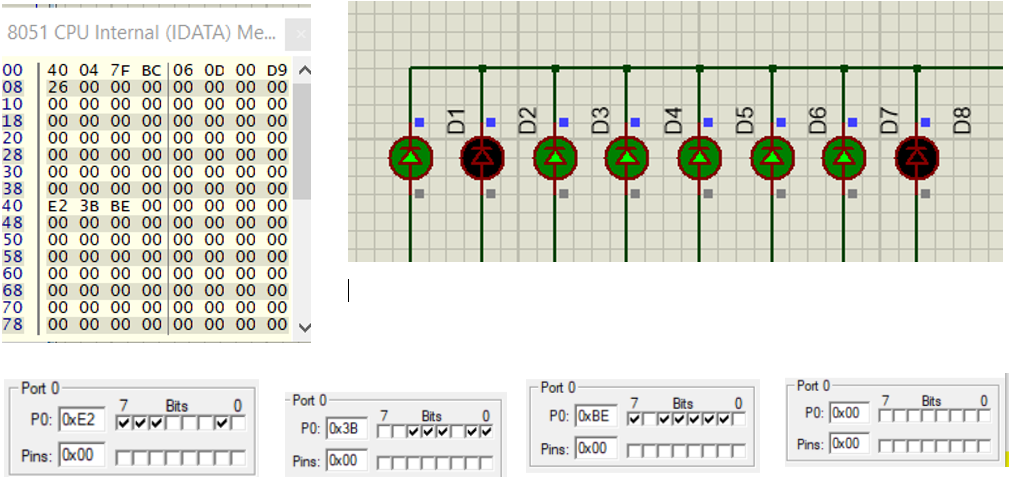
\includegraphics[scale=0.65,cframe=blue 0.5pt 3pt]{1.png}
	\textit{\caption{Addition of two hexadeciaml no.}}
\end{figure}

%%%%%%%%%%%%%%%%%%%%%%%


%%%%%222%%%%%%
\begin{Q}
	{
	Implement a subroutine that replaces the SWAP instruction using rotate right instructions.
	 Test your program on the contents of the accumulator when it contains the number 6BH. 
	}
\end{Q}

 
	\anscode{2a.asm}{2b.c}

\textbf{OUTPUT :\\}
	The upper and lower nibbles of accumulator are swaped without using the SWAP instruction. Hence, 6B H becomes B6 H once the swap is performed.

	\begin{figure}[H]
		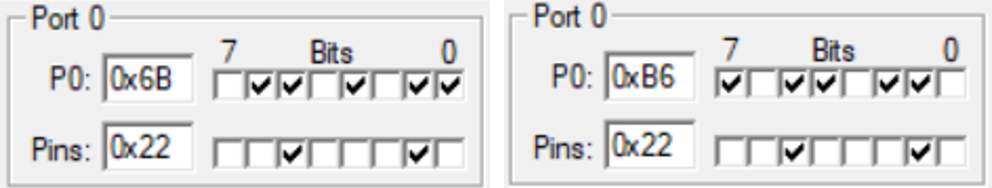
\includegraphics[scale=0.7,cframe=blue 0.5pt 3pt]{2.png}
		\textit{\caption{Swaping using rotate right}}
	\end{figure}
%%%%%%%%%%%%%%%%%%

%%%%%%%%%33333%%%%%%%
\begin{Q}
	{
		Multiply, by using looping and successive addition technique, 
		the data in RAM location 22H by the data in RAM location 15H and put the result in RAM locations 19H (low byte) and 1AH (high byte).
		 Data in 22H should be FFH and data in 15H should be DEH. 
	}
\end{Q}

 
	\anscode{3a.asm}{3b.c}


	\textbf{OUTPUT :\\}
	Multiplication of FF H and DE H is DD22 H
	\begin{figure}[H]
		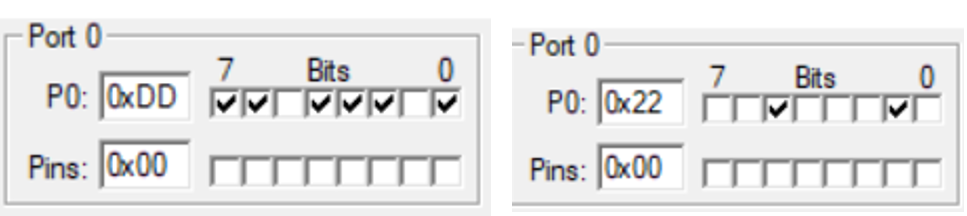
\includegraphics[scale=0.7,cframe=blue 0.5pt 3pt]{3.png}
		\textit{\caption{Multiplication using Addition}}
	\end{figure}
%%%%%%%%%%%%%%%%%%
\pagebreak

%%%%%44444%%%%
\begin{Q}
	{
		Divide, by using looping and successive subtraction technique, the data in RAM location 3EH by the number 12H;
		 put the quotient in R4 and remainder in R5. Data in 3EH should be AFH. 
	}
\end{Q}

 
	\anscode{4a.asm}{4b.c}
 

	\textbf{OUTPUT :\\}
	Dividing AF H by 12 H gives quotient = 9 H and remainder = D H,which are  stored in R4 and R5 register.

	\begin{figure}[H]
		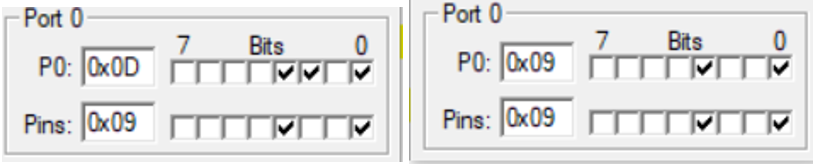
\includegraphics[scale=0.8,cframe=blue 0.5pt 3pt]{4.png}
		\textit{\caption{Division using Subtraction}}
	\end{figure}

%%%%%%%%%%%%%%%%%%
%%%%%55555%%%%
\begin{Q}
	{
		Store ten hexadecimal numbers in internal RAM starting from memory location 50H. The list of numbers to be used is: D6H, F2H, E4H, A8H, CEH, B9H, FAH, AEH, BAH, CCH. 
		Implement a subroutine that extracts both the smallest and largest numbers from the stored numbers. 
	}
\end{Q}

 
	\anscode{5a.asm}{5b.c}
 
	\textbf{OUTPUT :\\}
Among 10 stored Numbers Largest number = FA H and smallest number = A8 H.

	\begin{figure}[H]
		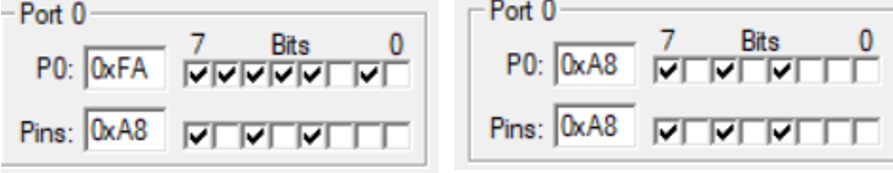
\includegraphics[scale=0.7,cframe=blue 0.5pt 3pt]{5.png}
		\textit{\caption{Finding largest and smallest number}}
	\end{figure}
%%%%%%%%%%%%%%%%%%
\pagebreak
%%%%%%66666%%%
\begin{Q}
	{
		Store ten hexadecimal numbers in internal RAM starting from memory location 60H. The list of numbers to be used is: A5H, FDH, 67H, 42H, DFH, 9AH, 84H, 1BH, C7H, 31H.
		 Implement a subroutine that orders the numbers in ascending order using bubble or any other sort algorithm and implement s 
		subroutine that order the numbers in descending order using selection sort algorithm. 
	}
\end{Q}

\large{\textsc{\\Bubble sort\\}}
 
	\anscode{6a1.asm}{6b1.c}

	\textbf{OUTPUT :\\}
	10 hexadecimal numbers sorted in ascending order using bubble sort algorithm

	\begin{figure}[H]
		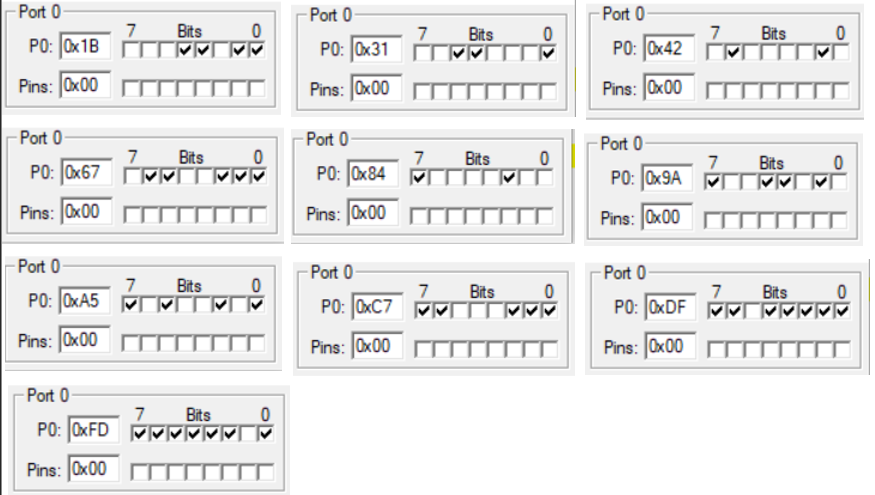
\includegraphics[scale=0.7,cframe=blue 0.5pt 3pt]{6a.png}
		\textit{\caption{Sorting in Ascending order using bubble sort}}
	\end{figure}

	\pagebreak
\large{\textsc{\\Selection Sort\\}}
 
	\anscode{6a2.asm}{6b2.c}
 


	\textbf{OUTPUT :\\}

	10 hexadecimal numbers sorted in descending order using selection sort algorithm.
	\begin{figure}[H]
		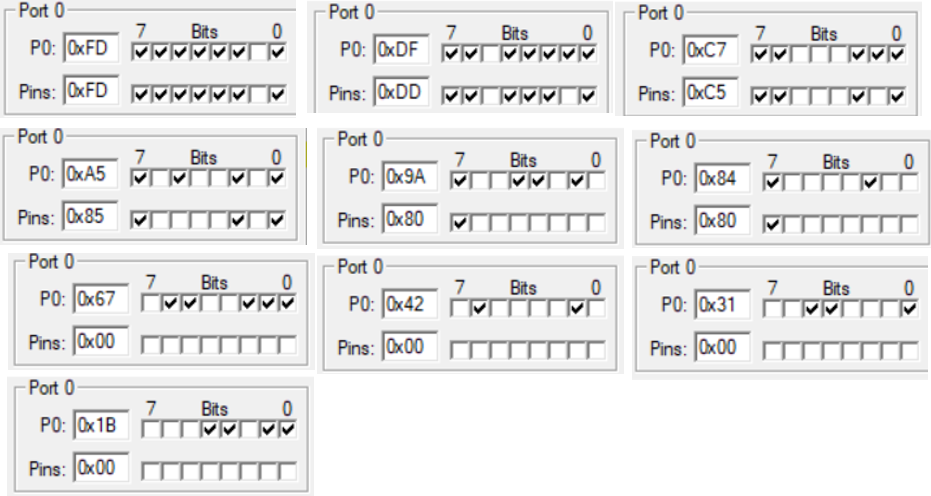
\includegraphics[scale=0.7,cframe=blue 0.5pt 3pt]{6b.png}
		\textit{\caption{Sorting in Decending order using Selection sort}}
	\end{figure}

%%%%%%%%%%%%%%%%%%
\pagebreak
%%%%%7777777%%%%
\begin{Q}
	{
		Store ten hexadecimal numbers in internal RAM starting from memory location 60H. The list of numbers to be used is: A5H, FDH, 67H, 42H, DFH, 9AH, 84H, 1BH, C7H, 31H.
		 Implement a subroutine that orders the numbers in ascending order using bubble or any other sort algorithm and implement subroutine that order the numbers in descending order using selection sort algorithm. 
	}
\end{Q}

 
	\anscode{7a.asm}{7b.c}
 


	\textbf{OUTPUT :\\}
	Only the prime numbers among 00 H to 20 H stored in memory location starting from 40H were to be shown.
	\begin{figure}[H]
		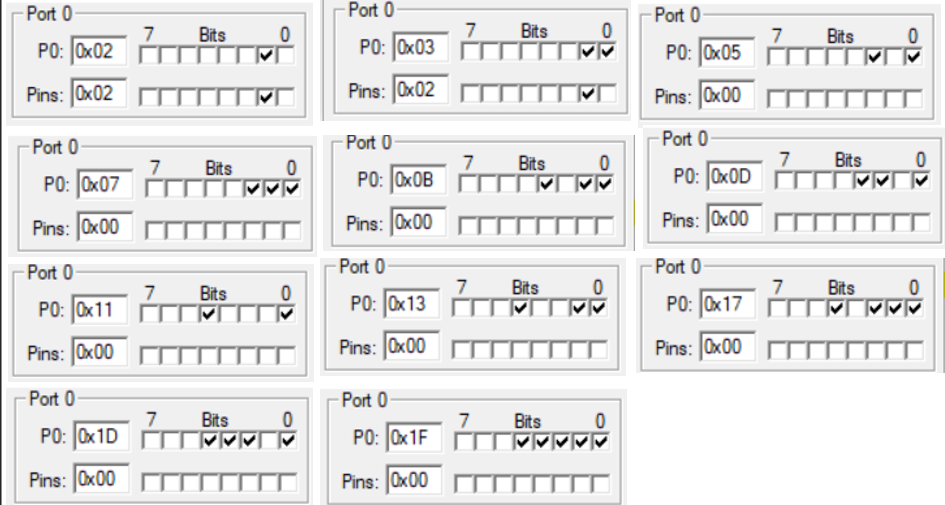
\includegraphics[scale=0.7,cframe=blue 0.5pt 3pt]{7.png}
		\textit{\caption{Extracting Prime numbers}}
	\end{figure}

%%%%%%%%%%%%%%%%%%
\pagebreak
%%%%%%888888%%%
\begin{Q}
	{
		Find the factorial of a number stored in R3. The value in R3 could be any number in the range from 00H to 05H.
		 Implement a subroutine that calculates the factorial.
		 The factorial needs to be represented in both hexadecimal and decimal formats. 
	}
\end{Q}

 
	\anscode{8a.asm}{8b.c}
 

\textbf{OUTPUT :\\}
Factorial of 5 is 78 H or 120 D.
	\begin{figure}[H]
		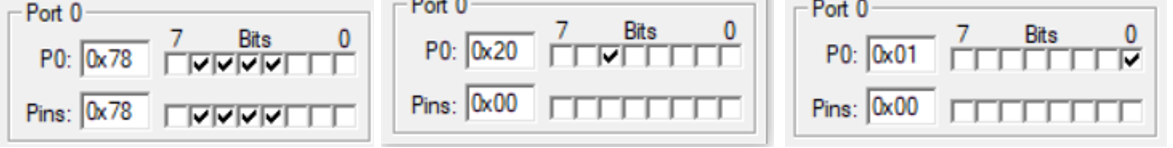
\includegraphics[scale=0.58,cframe=blue 0.5pt 3pt]{8.png}
		\textit{\caption{Finding Factorial of a number}}
	\end{figure}

%%%%%%%%%%%%%%%%%%

\section{Discussion \& Conclusion}
{In this Lab we perform Addition, substraction, rotation, multiplication, division, additional data manipulation,
 various logical oper ations based on flags and subroutine calls to be familiar with the 8051/52 microcontroller and
  basic programming approaches to 8051/52 MCUs.Keil IDE and Proteus Simulation Software were used to verify the result. Schematic diagram made in Proteus is included .
Codes of both language Assembly an embedded C is included int his lab report.

  }


\end{document}